\chapter{Domain Generalization} % Main chapter title
\label{DomainGeneralization} 

Machine learning systems often lack \emph{out-of-distribution generalization} which causes models to heavily rely on the training distribution and as a result don't perform very well when presented with irregular statistical qualities during testing. For example, this can be seen in application scenarios where intelligent systems don't generalize well across health centers if the training data was only collected in a single hospital \citep{Castro_2020, AlBadawy2018, PeroneBBC19} or when self-driving cars struggle under alternative lighting or weather conditions \citep{DaiG18, VolkMBH019}. Properties which are often interpreted falsely as part of the relevant feature set include backgrounds \citep{BeeryHP18}, textures \citep{GeirhosRMBWB19}, or racial biases \citep{StockC18}. Not only can a failure in capturing this domain shift lead to poor performance, but in safety-critical scenarios this can correspond to a large impact on people's lives. Due to the prevalence of this challenge for the wide-spread deployment of machine learning systems in diverse environments, many researchers tried to tackle this task with different approaches. In this chapter, we want to give a broad overview over the literature in \emph{domain generalization} and prepare the fundamentals for the following chapters. If you are already familiar with the field, you can safely skip this chapter and only familiarize yourself with the used notation.

\section{Problem formulation}
\label{sec:domain_gen_problem}

\paragraph{Supervised Learning}
In supervised learning we are aiming to optimize the predictions $\yy$ for the values $\yy \in \ys$ of a random variable $\yrandom$, when presented with values $\xx \in \xs$ of a random variable $\xrandom$. These predictions are generated with a model predictor $\f{\cdot}: \xs \rightarrow \ys$ that is parameterized by parameters $\p \in \ps$, usually the weights of a neural network,  and is assigning the predictions as $\ypred=\f{\cdot}$. To improve our predictions, we utilize a training dataset containing $n$ input-output pairs denoted as $\data=\left\{\left(\xxi, \yyi \right)\right\}_{i=1}^{n}$ where each sample $\sample$ is ideally drawn identically and independently distributed (i.i.d.) from a single joint probability distribution $\dist$. By using a loss term $\lossi{\ypred}{\yy}: \ys \times \ys \rightarrow \mathbb{R}^{+}$, which quantifies how different the prediction $\ypred$ is from the ground truth $\yy$, we would like to minimize the risk,
\begin{equation}
    \risk = \mathbb{E}_{\sample \sim \dist}\left[\lossi{\f{\xxi}}{\yyi}\right],
\end{equation}
of our model. Since we only have access to the distribution $\dist$ through a proxy in the form of the dataset $\data$, we are instead using Empirical Risk Minimization (ERM):
\begin{equation}
    \riske =\frac{1}{n} \sum_{i=1}^n \lossi{\f{\xxi}}{\yyi},
\end{equation}
by adding up the loss terms of each sample. One common choice for this loss term is the Cross-Entropy (CE) loss which is shown in \Cref{eq:cross_entropy}.
\begin{equation}
\label{eq:cross_entropy}
    \lterm_{ce}(\ypred_i, \yioh)=-\sum_{c=1}^{C} y_{i, c} \cdot \log \left(\hat{y}_{i, c}\right)
\end{equation}
Here, $\yioh$ is the one-hot vector representing the ground truth class, $\ypred_i$ is the \emph{softmax} output of the model, $y_{i, c}$ and $\hat{y}_{i, c}$ are the $c$-th dimension of $\ypred_i$ and $\yioh$ respectively.

The occurring minimization problem is then often solved through iterative gradient based optimization algorithms \eg \sgd{} \citep{Robbins1951} or \adam \citep{Kingma2015} which perform on-par with recent methods for the non-convex, continuous loss surfaces produced by modern machine learning problems and architectures \citep{schmidt2020descending}.

On top of that, the model predictor $\modelf$ can be decomposed into two functions as $\modelf = \classifier \circ \featureex$ where $\featureex: \xs \rightarrow \zs$ is an embedding into a feature space, hence sometimes called the feature extractor, and $\classifier: \zs \rightarrow \ys$ which is called the classifier since it is a prediction from the feature space to the output space \citep{gulrajani2020search, MotiianPAD17}. This often allows for a more concise mathematical notation.

\paragraph{Domain Generalization}
The problem of \emph{Domain generalization} (DG) builds on top of this framework, where now we have a set of training environments $\envs = \left\{\env_{1}, \ldots, \env_{s} \right\}$, also known as source domains, where each each environment $\env$ has an associated dataset $\data_{\env}=\left\{\left(\xxi^{\env}, \yyi^{\env}\right)\right\}_{i=1}^{n_{\env}}$ containing $n_\env$ i.i.d. samples from individual data distributions $\dist_\env$. Note that, while related, the environments have different joint distributions, \ie $\dist_{\env_i}\neq \dist_{\env_j} \;\forall i\neq j$. Here, $\xxi^\env \in \mathbb{R}^{m}$ is the $i$-th sample for environment $\env$ representing a $m$-dimensional feature vector (\ie an image in our case) and $\yyi^\env \in \ys$ is the corresponding ground truth class label over the $C$ possible classes. The one-hot vector representing the ground truth is denoted as $\yioh^\env$. To clear up some notation, we sometimes omit $\env$ where it is obvious. From these domains, we try to learn generic feature representations agnostic to domain changes to improve model performance \citep{seo2019learning}. Simply, we try to do \emph{out-of-distribution generalization} where our model aims to achieve good performance for an unseen test environment $\env_t$ sampled from the set of unseen environments $\tenvs = \left\{\env_{1}, \ldots, \env_{t}\right\}$ with $\envs \cap \tenvs =\emptyset$ based on statistical invariances across the observed training (source) and testing (target) domains \citep{gulrajani2020search, huang2020selfchallenging}. For that, we try to minimize the expected target risk of our model as:
\begin{equation}
\label{eq:domain_risk}
    \risk = \mathbb{E}_{(\xxi^{\env_t}, \yyi^{\env_t}) \sim \dist_{\env_t}}\left[\lossi{\f{\xxi^{\env_t}}} {\yyi^{\env_t}}\right].
\end{equation}
Since we don't have access to $\dist_{\env_{t}}$ during training, one simple approach is to assume that minimizing the risk over all source domains in $\envs$ achieves good generalization to the target domain. That is, we disregard the separated environments:
\begin{equation}
\label{eq:erm}
    \risk = \mathbb{E}_{(\xxi, \yyi) \sim \cup_{\env \in \envs} \dist_\env} \left[\lossi{\f{\xxi}} {\yyi} \right].
\end{equation}
Again, this can be written with the empirical risk as a simple sum over all the environments and their corresponding samples:
\begin{equation}
\label{eq:domain_risk_emp}
    \riske = \frac{1}{s} \sum_{\env \in \envs} \frac{1}{n_\env} \sum_{i=1}^{n_\env} \lossi{\f{\xxi^{\env}}} {\yyi^{\env}}.
\end{equation}
The difference of this approach when compared to ordinary supervised learning is summarized on a high-level in \Cref{tab:learning_setups}. It may also be helpful to think about a meta-distribution $\meta$ (real-world) generating source environment distributions $\dist_\env^\envs$ and unseen testing domain distributions $\mathcal{D}_\env^\tenvs$ as shown in \Cref{fig:meta_domain}.
\begin{figure}[htbp]
    \centering
    \begin{tikzpicture}[
            > = stealth, % arrow head style
            shorten > = 1pt, % don't touch arrow head to node
            auto,
            node distance = 3cm, % distance between nodes
            semithick % line style
        ]
    \tikzstyle{every state}=[
            draw = black,
            thick,
            fill = white,
            minimum size = 1cm
        ]

        \node[state] (meta) at (0,0) {\Large{$\meta$}};
        \node[state] (d1) at (-3,-2) {$\dist_{\env_1}^\envs$};
        \node[state] (d2) at (-1,-2) {$\dist_{\env_s}^\envs$};
        \node[state] (d3) at (1,-2) {$\dist_{\env_1}^\tenvs$};
        \node[state] (d4) at (3,-2) {$\dist_{\env_t}^\tenvs$};

        \path[->] (meta) edge node {} (d1);
        \path[->] (meta) edge node {} (d2);
        \path[->] (meta) edge node {} (d3);
        \path[->] (meta) edge node {} (d4);
        \path (d1) -- node[auto=false]{\ldots} (d2);
        \path (d3) -- node[auto=false]{\ldots} (d4);
    \end{tikzpicture}
    \caption[Meta-distribution $\meta$ generating source and unseen domain distributions]{Meta-distribution $\meta$ generating source environment distributions (left) and unseen environment distributions (right), adapted from: \citep{albuquerque2019generalizing}}
    \label{fig:meta_domain}
\end{figure}

\begin{table}[t]
    \centering
    \begin{tabular}{lll}
    \toprule
    \textbf{Setup} & \textbf{Training inputs}  & \textbf{Testing inputs} \\
    \midrule
        Generative learning & $U_{\env_1}$ & $\emptyset$ \\ 
        Unsupervised learning & $U_{\env_1}$ & $U_{\env_1}$  \\ 
        Supervised learning & $L_{\env_1}$ & $U_{\env_1}$ \\ 
        Semi-supervised learning & $L_{\env_1}, U_{\env_1}$ & $U_{\env_1}$ \\ 
        Multitask learning & $L_{\env_1}, \ldots, L_{\env_s}$ & $U_{\env_1}, \ldots, U_{\env_s}$ \\ 
        Continual (lifelong) learning & $L_{\env_1}, \ldots, L_{\env_\infty}$ & $U_{\env_1}, \ldots, U_{\env_\infty}$ \\ 
        Domain Adaptation & $L_{\env_1}, \ldots, L_{\env_s}, U_{\env_t}$ & $U_{\env_t}$ \\ 
        Transfer learning & $U_{\env_1}, \ldots, U_{\env_s}, L_{\env_t}$ & $U_{\env_t}$ \\ 
        \emph{Domain generalization} & $L_{\env_1}, \ldots, L_{\env_s}$ & $U_{\env_t}$ \\ 
    \bottomrule
    \end{tabular}
    \caption[Differences in learning setups]{Differences in learning setups adapted from: \citep{gulrajani2020search}. For each environment $\env$ the labeled and unlabeled datasets are denoted as $L_\env$ and $U_\env$ respectively.}
    \label{tab:learning_setups}
\end{table}

\paragraph{Homogeneous and Heterogeneous}
Sometimes, domain generalization is also divided into \emph{homogeneous} and \emph{heterogeneous} subtasks. In homogeneous DG we assume that all domains share the same label space $\ys^{\env_i} = \ys^{\env_j} = \ys^{\env_t}$, $\forall \env_i, \env_j \in \envs$. On the contrary, the more challenging heterogeneous DG allows for different label spaces $\ys^{\env_i} \neq \ys^{\env_j} \neq \ys^{\env_t}$ which can even be completely disjoint \citep{LiZYLSH19}. For this work, we assume the homogeneous setting.

\paragraph{Single- and Multi-Source}
There exist subtle differences within this task which are called \emph{single-} or \emph{multi-source domain generalization}. While multi-source domain generalization refers to the standard setting we have just outlined, single-source domain generalization is a more generic formulation \citep{zunino2020explainable}. Instead of relying on multiple training domains to learn models which generalize better, single-source domain generalization aims at learning these representations with access to only one source distribution. Hence, our training domains are restricted to $\envs = \left\{\env_1\right\}$, described by one dataset $\data_{\env_1}=\left\{\left(\xxi^{\env_1}, \yyi^{\env_1}\right)\right\}_{i=1}^{n_{\env_1}}$ and modeling a single source distribution $\dist_{\env_1}$. For example, this can be achieved by combining the different datasets or distributions similar to \Cref{eq:erm} or mathematically $\cup_{\env \in \envs} \dist_\env$. This is different from the ordinary supervised learning setup since we want to analyze the performance of the model under a clear domain-shift (\ie out-of-distribution generalization). Keep in mind, that strong regularization methods will also perform well on this subtask. These cross-over and related techniques are described in the following section.

\section{Related concepts and their differences}

As already introduced, members of the causality community might know the task of domain generalization under the term \emph{learning from multiple environments} \citep{arjovsky2019invariant, gulrajani2020search, PetBuhMei15} and researchers coming from deep learning might know it under \emph{learning from multiple domains}. While these two concepts refer to the same task, there exist quite a few related techniques which we want to highlight here and distinguish in their scope. In particular, we focus on ``Generic neural network regularization'' and ``Domain Adaptation'' since these are very closely related and sometimes hard to distinguish if at all. The overview in \Cref{tab:learning_setups}, however, includes even more learning setups to properly position this concept into the machine learning landscape.

\subsection{Generic Neural Network Regularization}

In theory, generic model regularization which aims to prevent neural networks from overfitting on the source domain, could also improve the domain generalization performance \citep{huang2020selfchallenging}. As such, methods like dropout \citep{SrivastavaHKSS14}, early stopping \citep{CaruanaLG00}, or weight decay \citep{NowlanH92} can have a positive effect on this task when deployed properly. Apart from regular dropout, where we randomly disable neurons in the training phase to stop them from co-adapting too much, a few alternative methods exist. These include dropping random  patches of input images (Cutout \& HaS) \citep{devries2017improved, SinghL17} or channels of the feature map (SpatialDropout) \citep{TompsonGJLB15}, dropping contiguous regions of the feature maps (DropBlock) \citep{GhiasiLL18}, dropping features of high activations across feature maps and channels (MaxDrop) \citep{ParkK16}, or generalizing the traditional dropout of single units to entire layers during training (DropPath) \citep{LarssonMS17}. There even exist methods like curriculum dropout \citep{MorerioCVVM17} which deploy scheduling for the dropout probability and therefore softly increase the amount of units to be suppressed layerwise during training. 

Generally, deploying some of these methods when aiming for out-of-distribution generalization can be a good idea and should definitely be considered for the task of domain generalization.


\subsection{Domain Adaptation}

\emph{Domain Adaptation} (DA) is often mentioned as a closely related task in domain generalization literature \citep{MotiianPAD17, VolpiM19, QiaoZP20}. When compared, domain adaptation has additional access to an unlabeled dataset from the target domain \citep{mancini2020, Csurka17}. Formally, aside from the set of source domains $\envs$ and the domain datasets $\data_\env$, as outlined in \Cref{sec:domain_gen_problem}, we have access to target samples $U_{\env_t} = \left\{\xx_1^{\env_t},\dots,\xx_{n_{\env_t}}^{\env_t}\right\}$ that are from the target domain $\xxi^{\env_t} \sim \dist_{\env_t}$ but their labels remain unknown in training since we want to predict them during testing. As a result, domain generalization is considered to be the harder problem of the two. This difference is also shown in \Cref{tab:learning_setups}.

Earlier methods in this space deploy hand-crafted features to reduce the difference between the source and the target domains \citep{ManciniPBC018}. Like that, \emph{instance-based methods} try to re-weight source samples according to target similarity \citep{GongGS13, HuangSGBS06, YamadaSR12} or \emph{feature-based methods} try to learn a common subspace \citep{FernandoHST13, GongSSG12, LongD0SGY13, BaktashmotlaghHLS13}. More recent works focus on \emph{deep domain adaptation} based on deep architectures where domain invariant features are learned utilizing supervised neural networks \citep{BousmalisTSKE16, CarlucciPCRB17, GaninL15, GhifaryKZBL16}, autoencoders \citep{ZengOWW14}, or generative adversarial networks (GANs) \citep{BousmalisSDEK17, ShrivastavaPTSW17, TzengHSD17}. These deep neural network based architectures significantly outperform the approaches for hand-crafted features \citep{ManciniPBC018}.

Even though domain adaptation and domain generalization both try to reduce the dataset bias, they are not compatible to each other \citep{GhifaryBKZ17}. Hence, domain adaptation methods often cannot be directly used for domain generalization or vice versa \citep{GhifaryBKZ17}. For this work, we don't rely on the simplifying assumptions of domain adaptation, but instead tackle the more challenging task of domain generalization.

\section{Previous Works}

Most commonly, work in \emph{domain generalization} can be divided into methods which try to \emph{learn invariant features}, combine domain specific models in a process called \emph{model ensembling}, pursue \emph{meta-learning}, or utilize \emph{data augmentation} to generate new domains or more robust representations.

Since literature in the domain generalization space is very broad, we utilized \citet[Appendix A]{gulrajani2020search} for an overview and to identify relevant literature while individually adding additional works and more detailed information where necessary.  

\subsection{Learning invariant features}
\label{sec:invariant_features}

Methods which try to learn invariant features typically minimize the difference between source domains. They assume that with this approach the features will be domain-invariant and therefore will have a good performance for unseen testing domains \citep{huang2020selfchallenging}.

Some of the earliest works on learning invariant features were \emph{kernel methods} applied by \citet{MuandetBS13}  where they look for a feature transformation that minimizes the across-domain dissimilarity between transformed feature distributions while preserving the functional relationship between original features and targets. In recent years, there have been approaches following a similar kernel based approach \citep{LiGTLT18, LiTGLLZT18}, sometimes while maximizing class separability \citep{Hu0CC19, GhifaryBKZ17}. As an early method, \citet{FangXR13} introduce Unbiased Metric Learning (UML) with a SVM metric that enforces the neighborhood of samples to contain samples with the same class label but from other training domains.

After that, \citet{GaninUAGLLML16} introduced Domain Adversarial Neural Networks (DANNs) utilizing neural network architectures to learn domain-invariant feature representations by adding a gradient reversal layer. Recently, their approach got extended to support statistical dependence between domains and class labels \citep{AkuzawaIM19} or considering one-versus-all adversaries to minimize pairwise divergences between source distributions \citep{albuquerque2019generalizing}. \citet{MotiianPAD17} use a siamese architecture to learn a feature transformation which tries to achieve semantical alignment of visual domains while maximally separating them. Other methods are also matching the feature covariance across source domains \citep{RahmanFBS20} or take an causal interpretation to match representations of features \citep{mahajan2020domain}. \citet{huang2020selfchallenging} have also shown that self-challenging (\ie dropping features with high gradient values at each epoch) works very well despite its simplicity. 

\citet{MatsuuraH20} use clustering techniques to split single-source domain generalization into different domains and then train a domain-invariant feature extractor via adversarial
learning. Other works have also deployed similar approaches based of adversarial strategies \citep{deng2020representation, Jia_2020_CVPR_SSDG}.

\citet{LiPWK18} deploy adversarial autoencoders with maximum mean discrepancy (MMD) \citep{GrettonBRSS12} to align the source distributions, \ie for distributions $\dist_{\env_1}$, $\dist_{\env_2}$ and a feature map $\varphi: \mathcal{X} \rightarrow \mathcal{H}$ where $\mathcal{H}$ is a reproducing kernel Hilbert space (RKHS) this measure is defined as \Cref{eq:mmd}.
\begin{equation}
\label{eq:mmd}
    \operatorname{MMD}(\dist_{\env_1}, \dist_{\env_2})=\left\|\mathbb{E}_{\sample \sim \dist_{\env_1}}[\varphi(\xxi^{\env_1}))]-\mathbb{E}_{\sample \sim \dist_{\env_2}}[\varphi(\xxi^{\env_2})]\right\|_{\mathcal{H}}
\end{equation}
\citet{ilse2019diva} extend the variational autoencoder \citep{KingmaW13} by introducing latent representations for environments $\zs_\env$, classes $\zs_\yy$ and residual variations $\zs_\xx$. Further, \citet{LiZYLSH19} use episodic training \ie they train a domain agnostic feature extractor $\featureex$ and classifier $\classifier$ by mismatching them with an equivalent trained on a specific domain $\featureex_\env$ and $\classifier_\env$ in combinations $(\featureex_{\env_1}, \classifier_{\env_2}, \xx^{\env_2}_i)$ and $(\featureex_{\env_2}, \classifier_{\env_1}, \xx^{\env_2}_i)$ and letting them predict data outside of the trained domain $\env_1 \neq \env_2$. \citet{piratla2020efficient} also learn domain specific and common components but the domain specific parts are discarded after training. \citet{li2020sequential} deploy a lifelong sequential learning strategy.

\subsection{Model ensembling}

Some methods try to associate model parameters with each of the training domains and combine them, often together with shared parameters, in a meaningful matter to improve generalization to the test domain. Commonly, the amount of models in these type of architectures grow linearly with the number of source domains. 

The first work to pose the problem of domain generalization and analyze it was \citet{BlanchardLS11}. In there, they use classifiers for each sample $\xx^\env$  denoted as $\f{\xx^\env, \mu^\env}$ where $\mu^\env$ corresponds to a kernel mean embedding \citep{MuandetFSS17}. For theoretical analysis on such methods please see \citet{an2019generalization} and \citet{blanchard2017domain}. Later on, \citet{KhoslaZMET12} combine global weights $\p$ with local domain biases $\Delta_\env$ to learn one max-margin linear classifier (SVM) per domain as $\p_\env = \p + \Delta_\env$ and finally combine them, which has recently been extended to neural network settings by adding an additional dimension describing the training domains to the parameter tensors \citep{LiYSH17}. \citet{GhifaryKZB15} propose a Multi-task Autoencoder (MTAE) with shared parameters to the hidden state and domain-specific parameters for each of the training domains. Further, \citet{ManciniBCR18} use domain-specific batch-normalization \citep{IoffeS15} layers and then linearly combine them using a softmax domain classifier. Other works utilize other domain specific normalization techniques \citep{seo2019learning}, linearly combine domain-specific predictors \citep{ManciniBC018}, or use more elaborate aggregation strategies to combine these \citep{DInnocenteC18}. \citet{DingF18} use multiple
domain-specific deep neural networks with a structured low-rank constraint and a domain-invariant deep neural network to generalize to the target domain. There have also been works which assign weights to minibatches depending on their respective error to the training distributions \citep{HuNSS18, sagawa2019distributionally}. \citet{jin2020feature} use attention mechanisms to allign the features of the different training domains.

\subsection{Meta-learning}
\emph{Meta-learning} approaches provide algorithms which tackle the problem of  \emph{learning  to learn} \citep{1998TP, SchmidhuberZW97}.
 As such, \citet{FinnAL17} propose a Model-Agnostic Meta-Learning (MAML) algorithm which is able to quickly learn new tasks with fine-tuning. \citet{LiYSH18} adapt this algorithm for domain generalization (no fine-tuning) such that we can adapt to new domains by utilizing the meta-optimization objective which ensures that steps to improve training domain performance should also improve testing domain performance. Both approaches are not bound to a specific architecture and can therefore be deployed for a wide variety of learning tasks. These approaches recently got extended by two regularizers that encourage general knowledge about inter-class relationships and domain-independent class-specific cohesion \citep{DouCKG19}, to instances of domain generalization where the label space varies from domain to domain \citep{LiYZH19}, or meta-learning a regularizer which encourages across-domain performance \citep{BalajiSC18}.

\subsection{Data Augmentation}
\emph{Data Augmentation} remains a competitive method for generalizing to unseen domains \citep{zhang2019unseen}. Works in this segment try to extend the source environments to a wider range of domains by augmenting the available training environments. However, to deploy an efficient procedure for that, human experts need to consider the data at hand to develop a useful routine \citep{gulrajani2020search}.

Several works have used the \textsc{mixup} \citep{ZhangCDL18} algorithm as a method to merge samples from different domains \citep{XuZNLWTZ20, yan2020improve, WangLK20, mancini2020}. Other works have also tried removing textural information from images \citep{WangHLX19} or shifting it more towards shapes \citep{nam2019reducing, asadi2019shape}. \citet{CarlucciDBCT19} used jigsaw puzzles of image patches as a classification task to show that this improves domain generalization while \citet{VolpiNSDMS18} demonstrate that adversarial data augmentation on a single domain is sufficient. Further, \citet{VolpiM19} use popular image transformations (\eg brightness, contrast, sharpness) with differing intensity levels to train a more robust model or \citet{somavarapu2020frustratingly} use other stylizing techniques. Several methods also utilize GANs to augment the available training data  \citep{RahmanFBS19, ZhouYHX20, ShankarPCCJS18} or use other methods to generate synthetic domains \citep{zhou2020learning}. \citet{QiaoZP20} deploy an adversarial domain augmentation approach using a Wasserstein Auto-Encoder \citep{TolstikhinBGS18}.

\section{Common Datasets}
There exist several datasets which are commonly used in domain generalization research. Here, we want to introduce the most popular choices as well as interesting datasets to consider. We give an overview over \emph{Rotated MNIST}, \emph{Colored MNIST}, \emph{Office-Home}, \emph{VLCS}, \emph{PACS}, \emph{Terra Incognita}, \emph{DomainNet}, and \emph{ImageNet-C}. Currently, the most popular choices include ``PACS'', ``VLCS'', and ``Office-Home''.

\subsection{Rotated MNIST}
The rotated MNIST (RMNIST) dataset \citep{GhifaryKZB15} is a variation of the original MNIST dataset \citep{lecun-mnisthandwrittendigit-2010} where each digit got rotated by degrees $\{0, 15, 30, 45, 60, 75\}$. Each rotation angle represents one domain as shown in \Cref{tab:common_examples} for classes ``2'' and ``4''. The overall dataset in \citet{gulrajani2020search} includes \num{70000} images from $10$ homogeneous classes ($0-9$) each with dimension $1\times28\times28$.

\begin{table}[htbp]
    \centering
    \begin{tabularx}{\textwidth}{lcYYYYYYYY}
    \toprule
    \textbf{Dataset}  & \textbf{Reference} & $\env_1$   &  $\env_2$ & $\env_3$ & $\env_4$ & $\env_5$ & $\env_6$ & $\dots$ & $\env_{75}$ \\
    \midrule
    \multirow{7}{*}{\textbf{ImageNet-C}}  & \multirow{7}{*}{\textbf{\citep{HendrycksD19}}} & \domainsize{Shot Noise} &     \domainsize{Impulse Noise} & \domainsize{Defocus Blur} & \domainsize{Snow} & \domainsize{Fog} & \domainsize{Brightness}  & &  \domainsize{Pixelate}   \\
    & & 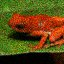
\includegraphics[height=\imagequadsize, width=\imagequadsize]{Figures/Chapter2/ImageNetC/shot_noise_class1.JPEG} &  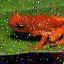
\includegraphics[height=\imagequadsize, width=\imagequadsize]{Figures/Chapter2/ImageNetC/impulse_noise_class1.JPEG} &  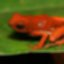
\includegraphics[height=\imagequadsize, width=\imagequadsize]{Figures/Chapter2/ImageNetC/defocus_blur_class1.JPEG} & 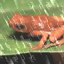
\includegraphics[height=\imagequadsize, width=\imagequadsize]{Figures/Chapter2/ImageNetC/snow_class1.JPEG} &  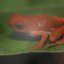
\includegraphics[height=\imagequadsize, width=\imagequadsize]{Figures/Chapter2/ImageNetC/fog_class1.JPEG} & 
       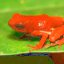
\includegraphics[height=\imagequadsize, width=\imagequadsize]{Figures/Chapter2/ImageNetC/brightness_class1.JPEG} & $\dots$ & 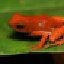
\includegraphics[height=\imagequadsize, width=\imagequadsize]{Figures/Chapter2/ImageNetC/pixelate_class1.JPEG} \\
        & & 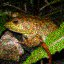
\includegraphics[height=\imagequadsize, width=\imagequadsize]{Figures/Chapter2/ImageNetC/shot_noise_class2.JPEG} &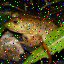
\includegraphics[height=\imagequadsize, width=\imagequadsize]{Figures/Chapter2/ImageNetC/impulse_noise_class2.JPEG} & 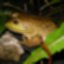
\includegraphics[height=\imagequadsize, width=\imagequadsize]{Figures/Chapter2/ImageNetC/defocus_blur_class2.JPEG} & 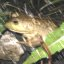
\includegraphics[height=\imagequadsize, width=\imagequadsize]{Figures/Chapter2/ImageNetC/snow_class2.JPEG} & 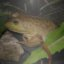
\includegraphics[height=\imagequadsize, width=\imagequadsize]{Figures/Chapter2/ImageNetC/fog_class2.JPEG} &
       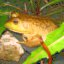
\includegraphics[height=\imagequadsize, width=\imagequadsize]{Figures/Chapter2/ImageNetC/brightness_class2.JPEG} & $\dots$ & 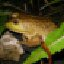
\includegraphics[height=\imagequadsize, width=\imagequadsize]{Figures/Chapter2/ImageNetC/pixelate_class2.JPEG} \\
       \addlinespace
        %%
       \multirow{7}{*}{\textbf{Rotated MNIST}}  & \multirow{7}{*}{\textbf{\citep{GhifaryKZB15}}} & \domainsize{$0^\circ$} & \domainsize{$15^\circ$} & \domainsize{$30^\circ$} & \domainsize{$45^\circ$} & \domainsize{$60^\circ$} & \domainsize{$75^\circ$} && \\
       & & 
\includegraphics[height=\imagequadsize, width=\imagequadsize]{Figures/Chapter2/RMNIST/RotatedMNIST_env00_2_idx470_class2.png} &  
\includegraphics[height=\imagequadsize, width=\imagequadsize]{Figures/Chapter2/RMNIST/RotatedMNIST_env115_6_idx8084_class2.png} &  
\includegraphics[height=\imagequadsize, width=\imagequadsize]{Figures/Chapter2/RMNIST/RotatedMNIST_env230_23_idx3711_class2.png} & 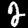
\includegraphics[height=\imagequadsize, width=\imagequadsize]{Figures/Chapter2/RMNIST/RotatedMNIST_env345_9_idx11212_class2.png} &  
\includegraphics[height=\imagequadsize, width=\imagequadsize]{Figures/Chapter2/RMNIST/RotatedMNIST_env460_11_idx7785_class2.png} & 
       
\includegraphics[height=\imagequadsize, width=\imagequadsize]{Figures/Chapter2/RMNIST/RotatedMNIST_env575_27_idx3863_class2.png} && \\
        & & 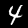
\includegraphics[height=\imagequadsize, width=\imagequadsize]{Figures/Chapter2/RMNIST/RotatedMNIST_env00_19_idx5269_class4.png} &
\includegraphics[height=\imagequadsize, width=\imagequadsize]{Figures/Chapter2/RMNIST/RotatedMNIST_env115_8_idx7608_class4.png} & 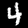
\includegraphics[height=\imagequadsize, width=\imagequadsize]{Figures/Chapter2/RMNIST/RotatedMNIST_env230_18_idx2042_class4.png} & 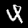
\includegraphics[height=\imagequadsize, width=\imagequadsize]{Figures/Chapter2/RMNIST/RotatedMNIST_env345_7_idx6290_class4.png} & 
\includegraphics[height=\imagequadsize, width=\imagequadsize]{Figures/Chapter2/RMNIST/RotatedMNIST_env460_6_idx1791_class4.png} &
       
\includegraphics[height=\imagequadsize, width=\imagequadsize]{Figures/Chapter2/RMNIST/RotatedMNIST_env575_14_idx11054_class4.png} & & \\
       \addlinespace
       %%
       \multirow{7}{*}{\textbf{DomainNet}} &  \multirow{7}{*}{\textbf{\citep{PengBXHSW19}}} & \domainsize{Clipart} & \domainsize{Graphic} & \domainsize{Painting} & \domainsize{Draw} & \domainsize{Photo} & \domainsize{Sketch}  & & \\
       & & 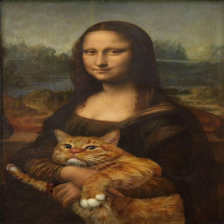
\includegraphics[height=\imagequadsize, width=\imagequadsize]{Figures/Chapter2/DomainNet/DomainNet_env0clipart_4_idx283_class2.png} & 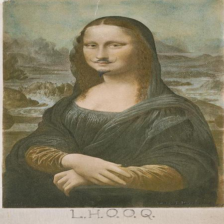
\includegraphics[height=\imagequadsize, width=\imagequadsize]{Figures/Chapter2/DomainNet/DomainNet_env1infograph_8_idx378_class2.png} & 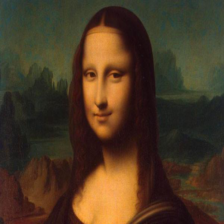
\includegraphics[height=\imagequadsize, width=\imagequadsize]{Figures/Chapter2/DomainNet/DomainNet_env2painting_41_idx507_class2.png} &  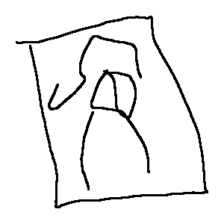
\includegraphics[height=\imagequadsize, width=\imagequadsize]{Figures/Chapter2/DomainNet/DomainNet_env3quickdraw_30_idx1326_class2.png} &  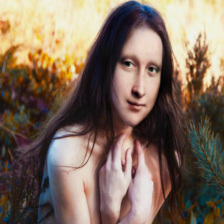
\includegraphics[height=\imagequadsize, width=\imagequadsize]{Figures/Chapter2/DomainNet/DomainNet_env4real_9_idx1117_class2.png} &  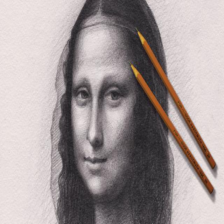
\includegraphics[height=\imagequadsize, width=\imagequadsize]{Figures/Chapter2/DomainNet/DomainNet_env5sketch_28_idx421_class2.png}  & & \\
       &  & 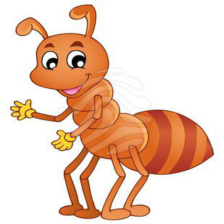
\includegraphics[height=\imagequadsize, width=\imagequadsize]{Figures/Chapter2/DomainNet/DomainNet_env0clipart_1_idx1098_class9.png} & 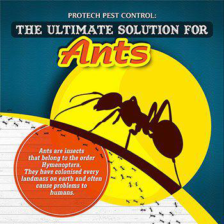
\includegraphics[height=\imagequadsize, width=\imagequadsize]{Figures/Chapter2/DomainNet/DomainNet_env1infograph_39_idx689_class9.png} & 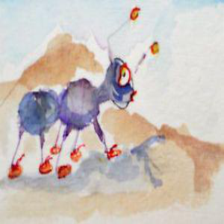
\includegraphics[height=\imagequadsize, width=\imagequadsize]{Figures/Chapter2/DomainNet/DomainNet_env2painting_25_idx2262_class9.png} & 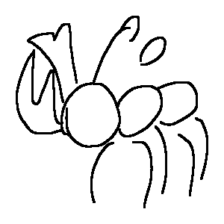
\includegraphics[height=\imagequadsize, width=\imagequadsize]{Figures/Chapter2/DomainNet/DomainNet_env3quickdraw_7_idx4907_class9.png} & 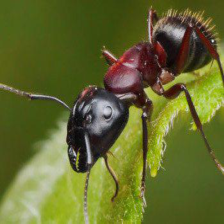
\includegraphics[height=\imagequadsize, width=\imagequadsize]{Figures/Chapter2/DomainNet/DomainNet_env4real_34_idx3532_class9.png} & 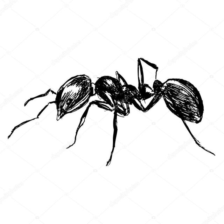
\includegraphics[height=\imagequadsize, width=\imagequadsize]{Figures/Chapter2/DomainNet/DomainNet_env5sketch_0_idx1772_class9.png}  & & \\
       \addlinespace
       %%
       \multirow{7}{*}{\textbf{Office-Home}} & \multirow{7}{*}{\textbf{\citep{VenkateswaraECP17}}} & \domainsize{Art} & \domainsize{Clipart} & \domainsize{Product} & \domainsize{Real} & &  & & \\
       & & 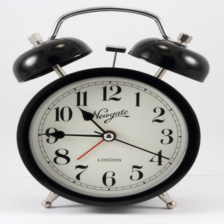
\includegraphics[height=\imagequadsize, width=\imagequadsize]{Figures/Chapter2/OfficeHome/OfficeHome_env0Art_1_idx61_class0.png} & 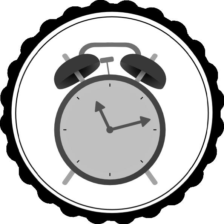
\includegraphics[height=\imagequadsize, width=\imagequadsize]{Figures/Chapter2/OfficeHome/OfficeHome_env1Clipart_5_idx24_class0.png} & 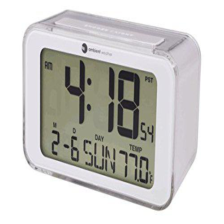
\includegraphics[height=\imagequadsize, width=\imagequadsize]{Figures/Chapter2/OfficeHome/OfficeHome_env2Product_14_idx67_class0.png} & 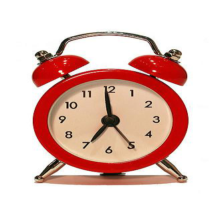
\includegraphics[height=\imagequadsize, width=\imagequadsize]{Figures/Chapter2/OfficeHome/OfficeHome_env3Real World_44_idx13_class0.png} & &  & & \\
        & & 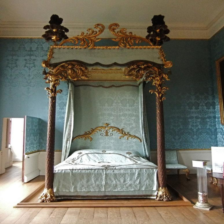
\includegraphics[height=\imagequadsize, width=\imagequadsize]{Figures/Chapter2/OfficeHome/OfficeHome_env0Art_18_idx176_class3.png} & 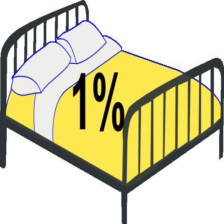
\includegraphics[height=\imagequadsize, width=\imagequadsize]{Figures/Chapter2/OfficeHome/OfficeHome_env1Clipart_12_idx199_class3.png} & 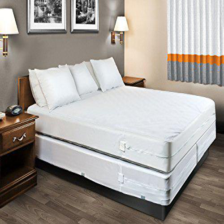
\includegraphics[height=\imagequadsize, width=\imagequadsize]{Figures/Chapter2/OfficeHome/OfficeHome_env2Product_19_idx261_class3.png} & 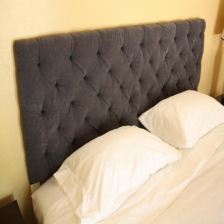
\includegraphics[height=\imagequadsize, width=\imagequadsize]{Figures/Chapter2/OfficeHome/OfficeHome_env3Real World_20_idx300_class3.png} & &  & & \\
        \addlinespace
        %%
       \multirow{7}{*}{\textbf{VLCS}} & \multirow{7}{*}{\textbf{\citep{FangXR13}}} & \domainsize{V} & \domainsize{L} & \domainsize{C} & \domainsize{S} & &  & & \\ 
       & & 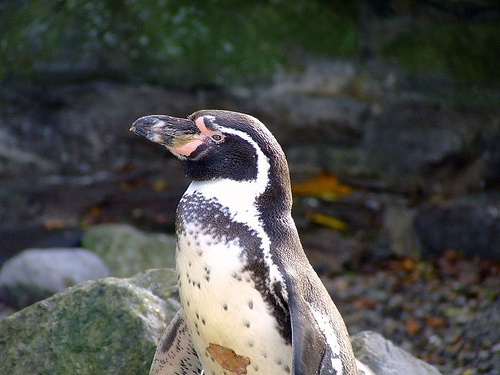
\includegraphics[height=\imagequadsize, width=\imagequadsize]{Figures/Chapter2/VLCS/voc_bird.jpg}  &  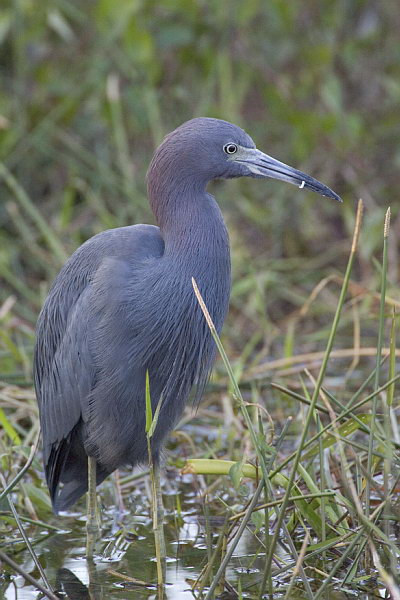
\includegraphics[height=\imagequadsize, width=\imagequadsize]{Figures/Chapter2/VLCS/labelme_bird.jpg} & 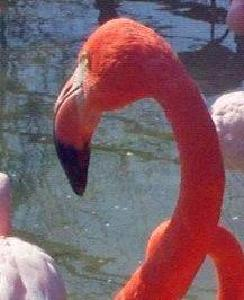
\includegraphics[height=\imagequadsize, width=\imagequadsize]{Figures/Chapter2/VLCS/caltech_bird.jpg} & 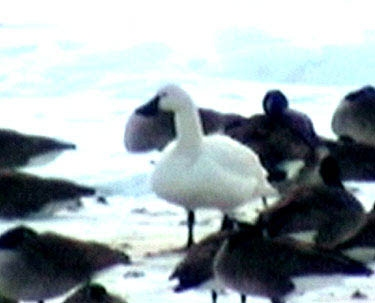
\includegraphics[height=\imagequadsize, width=\imagequadsize]{Figures/Chapter2/VLCS/sun_bird.jpg} & &  & & \\
       & & \includegraphics[height=\imagequadsize, width=\imagequadsize]{Figures/Chapter2/VLCS/voc_car.jpg} & \includegraphics[height=\imagequadsize, width=\imagequadsize]{Figures/Chapter2/VLCS/labelme_car.jpg} & \includegraphics[height=\imagequadsize, width=\imagequadsize]{Figures/Chapter2/VLCS/caltech_car.jpg} & \includegraphics[height=\imagequadsize, width=\imagequadsize]{Figures/Chapter2/VLCS/sun_car.jpg} & &  & & \\
       \addlinespace
       %%
       \multirow{7}{*}{\textbf{Terra Incognita}} & \multirow{7}{*}{\textbf{\citep{BeeryHP18}}} & \domainsize{L100} & \domainsize{L38} & \domainsize{L43} & \domainsize{L46} & &  & & \\ 
       & & \includegraphics[height=\imagequadsize, width=\imagequadsize]{Figures/Chapter2/TerraIncognita/TerraIncognita_env0location_100_22_idx685_class4.png} &  \includegraphics[height=\imagequadsize, width=\imagequadsize]{Figures/Chapter2/TerraIncognita/TerraIncognita_env1location_38_5_idx2429_class4.png} &
       \includegraphics[height=\imagequadsize, width=\imagequadsize]{Figures/Chapter2/TerraIncognita/TerraIncognita_env2location_43_45_idx2058_class4.png} &  \includegraphics[height=\imagequadsize, width=\imagequadsize]{Figures/Chapter2/TerraIncognita/TerraIncognita_env3location_46_6_idx2012_class4.png} & &  & & \\
       & & \includegraphics[height=\imagequadsize, width=\imagequadsize]{Figures/Chapter2/TerraIncognita/TerraIncognita_env0location_100_0_idx823_class5.png} & \includegraphics[height=\imagequadsize, width=\imagequadsize]{Figures/Chapter2/TerraIncognita/TerraIncognita_env1location_38_35_idx2747_class5.png} & \includegraphics[height=\imagequadsize, width=\imagequadsize]{Figures/Chapter2/TerraIncognita/TerraIncognita_env2location_43_38_idx2211_class5.png} & \includegraphics[height=\imagequadsize, width=\imagequadsize]{Figures/Chapter2/TerraIncognita/TerraIncognita_env3location_46_37_idx2142_class5.png} & &  & & \\
       \addlinespace
       %%
       \multirow{7}{*}{\textbf{PACS}} & \multirow{7}{*}{\textbf{\citep{LiYSH17}}}  & \domainsize{Art} & \domainsize{Cartoon} & \domainsize{Photo} & \domainsize{Sketch} & &  & & \\
       & & \includegraphics[height=\imagequadsize, width=\imagequadsize]{Figures/Chapter2/PACS/dog_1.jpg} &  \includegraphics[height=\imagequadsize, width=\imagequadsize]{Figures/Chapter2/PACS/dog_2.jpg} &  \includegraphics[height=\imagequadsize, width=\imagequadsize]{Figures/Chapter2/PACS/dog_3.jpg} &  \includegraphics[height=\imagequadsize, width=\imagequadsize]{Figures/Chapter2/PACS/dog_4.png} & &  & & \\
       & & \includegraphics[height=\imagequadsize, width=\imagequadsize]{Figures/Chapter2/PACS/elephant_1.jpg} & \includegraphics[height=\imagequadsize, width=\imagequadsize]{Figures/Chapter2/PACS/elephant_2.jpg} & \includegraphics[height=\imagequadsize, width=\imagequadsize]{Figures/Chapter2/PACS/elephant_3.jpg} & \includegraphics[height=\imagequadsize, width=\imagequadsize]{Figures/Chapter2/PACS/elephant_4.png} & &  & & \\
       \addlinespace
       %%
       \multirow{7}{*}{\textbf{Colored MNIST}} & \multirow{7}{*}{\textbf{\citep{arjovsky2019invariant}}} & \domainsize{$\plus90\%$} & \domainsize{$\plus80\%$} & \domainsize{$\minus90\%$} & & &  & & \\
       & & \includegraphics[height=\imagequadsize, width=\imagequadsize]{Figures/Chapter2/CMNIST/ColoredMNIST_env00.1_18_idx12999_class0.png} &  \includegraphics[height=\imagequadsize, width=\imagequadsize]{Figures/Chapter2/CMNIST/ColoredMNIST_env10.2_11_idx22249_class0.png} & \includegraphics[height=\imagequadsize, width=\imagequadsize]{Figures/Chapter2/CMNIST/ColoredMNIST_env20.9_1_idx13997_class0.png} & & &  & & \\
        & & \includegraphics[height=\imagequadsize, width=\imagequadsize]{Figures/Chapter2/CMNIST/ColoredMNIST_env00.1_8_idx9692_class1.png} & \includegraphics[height=\imagequadsize, width=\imagequadsize]{Figures/Chapter2/CMNIST/ColoredMNIST_env10.2_5_idx15365_class1.png} & \includegraphics[height=\imagequadsize, width=\imagequadsize]{Figures/Chapter2/CMNIST/ColoredMNIST_env20.9_9_idx7793_class1.png}  & & &  & & \\
        \addlinespace
    \bottomrule
    \end{tabularx}
    \caption{Samples for two different classes across domains for popular datasets}
    \label{tab:common_examples}
\end{table}

\subsection{Colored MNIST}

The colored MNIST (CMNIST) dataset \citep{arjovsky2019invariant} is another variation of the original MNIST dataset \citep{lecun-mnisthandwrittendigit-2010}. The grasyscale images of MNIST got colored in red and green. The respective label corresponds to a combination of digit and color where the color correlates to the class label with factors $\{0.1,0.2,0.9\}$ as domains and the digit has a constant correlation of $0.75$. Since this is a synthetic dataset, one can choose different, or more, factors for the domains. We report these numbers since they are used in \citet{gulrajani2020search, arjovsky2019invariant}. Since the correlation factor between color and label varies between domains, this dataset aims at getting rid of color as a predictive feature to improve generalization \citep{arjovsky2019invariant}.

To construct the dataset \citet{arjovsky2019invariant} first assign a initial label $\Tilde{y} = 0$ for digit $0-4$ and $\Tilde{y} = 1$ for digit $5-9$. This initial label is then flipped with a probability of $25\%$ to obtain the final label $y$. Finally, we obtain the color $z$ by flipping the label $y$ with probabilities $p^d \in \{0.1,0.2,0.9\}$ depending on the domain. The image is then colored red for $z=1$ or green for $z=0$ \citep{arjovsky2019invariant}. Samples for both classes across domains can be seen in \Cref{tab:common_examples}.

Overall, the dataset in \citet{gulrajani2020search} contains \num{70000} images from $2$ homogeneous classes (green \& red) of dimension $2 \times 28 \times 28$.  


\subsection{Office-Home}
The Office-Home dataset \citep{VenkateswaraECP17}  provides \num{15588} images from $65$ categories across $4$ domains. The domains include \emph{Art}, \emph{Clipart}, \emph{Products} (objects without a background), and \emph{Real-World} (captured with a regular camera). Samples from these domains for the classes ``alarm-clock'' and ``bed'' can be seen in \Cref{tab:common_examples}. On average, each class contains around $70$ images with a maximum of $99$ images in a category \citep{VenkateswaraECP17}. In \citet{gulrajani2020search} they use dimension $3 \times 224 \times 224$ for each image. 


\subsection{VLCS}

The VLCS dataset \citep{FangXR13} is a dataset which utilizes photographic datasets as individual domains. As such, it contains the domains \emph{PASCAL VOC} (V) \citep{EveringhamGWWZ10}, \emph{LabelMe} (L) \citep{RussellTMF08}, \emph{Caltech101} (C) \citep{Fei-FeiFP07}, and \emph{SUN09} (S) \citep{ChoiLTW10}. In total, there are \num{10729} images from $5$ classes. Samples for the classes ``bird'' and ``car'' can be seen in \Cref{tab:common_examples}. In \citet{gulrajani2020search} they use the dimension $3 \times 224 \times 224$ for each image. 

\subsection{PACS}
The PACS dataset \citep{LiYSH17} consists of images from different domains including \emph{photo} (P), \emph{art} (A), \emph{cartoon} (C) and \emph{sketch} (S) as individual domains. As such, it extends the previously photo-dominated data sets in domain generalization \citep{LiYSH17}. It includes $7$ homogeneous classes (dog, elephant, giraffe, guitar, horse, house, person) across the $4$ previously mentioned domains. \Cref{tab:common_examples} shows samples from the ``dog'' and ``elephant'' class across all domains. 

In total, PACS contains \num{9991} images which got obtained by intersecting classes from Caltech256 (Photo), Sketchy (Photo, Sketch) \citep{SangkloyBHH16}, TU-Berlin (Sketch) \citep{EitzHA12} and Google Images (Art, Cartoon, Photo) \citep{LiYSH17}.


\subsection{Terra Incognita}
The Terra Incognita dataset is a subset of the initial caltech camera traps dataset proposed by \citet{BeeryHP18}. It contains photographs of wild animals taken by camera traps at different locations (IDs: $38$, $43$, $46$, $100$) which represent the domains. As such, the version used by \citet{gulrajani2020search} contains \num{24788} images of $10$ classes, each with size $3\times 224 \times 224$. Samples from two different classes can be seen in \Cref{tab:common_examples}. The chosen locations represent the Top-4 locations with the largest number of images, each with more than \num{4000} images. 

The main data challenges which arise in this dataset include illumination, motion blur, size of the region of interest, occlusion, camouflage, and perspective \citep{BeeryHP18}. This includes animals not always being salient or them being small or far from the camera which results in only partial views of the animals' body being available \citep{BeeryHP18}. 

\subsection{DomainNet}

The DomainNet dataset \citep{PengBXHSW19} contains six domains: \emph{clipart} (\num{48129} images), \emph{infographic} (\num{51605} images), \emph{painting} (\num{72266} images), \emph{quickdraw} (\num{172500} images), \emph{real} (\num{172947} images), and \emph{sketch} (\num{69128} images) for $345$ classes. In total, it contains \num{586575} images  which got accumulated by searching a category with a domain name in multiple image search engines and, as an exception, players of the game ``Quick Draw!'' for the quickdraw domain \citep{PengBXHSW19}.

To secure the quality of the dataset, they hired $20$ annotators for a total of \num{2500} hours to filter out falsely labeled images \citep{PengBXHSW19}. Each category has an average of $150$ images for the domains \emph{clipart} and \emph{infographic}, $220$ images for \emph{painting} and \emph{sketch}, and $510$ for \emph{real} \citep{PengBXHSW19}.

\subsection{ImageNet-C}
The ImageNet-C dataset \citep{HendrycksD19} contains images out of ImageNet \citep{RussakovskyDSKS15} permutated according to $15$ corruption types each with $5$ levels of severity which results in $75$ domains. The type of corruptions are out of the categories ``noise'', ``blur'', ``weather'', and ``digital'' \citep{HendrycksD19}. \Cref{tab:common_examples} shows a few of the available corruptions at severity $3$ for the same image sample of two different classes. As their corruptions, they provide \emph{Gaussian Noise}, \emph{Shot Noise}, \emph{Impulse Noise}, \emph{Defocus Blur}, \emph{Frosted Glass Blur}, \emph{Motion Blur}, \emph{Zoom Blur}, \emph{Snow}, \emph{Frost}, \emph{Fog}, \emph{Brightness}, \emph{Contrast}, \emph{Elastic}, \emph{Pixelate}, and \emph{JPEG} \citep{HendrycksD19}. 

Overall, the dataset provides all \num{1000} ImageNet classes where each image has the standard dimension of $3 \times 224 \times 224$.

\section{Considerations regarding model validation}
\label{sec:considerations}

In traditional supervised learning setups, we train our model on the training dataset, validate its hyperparameters (\eg number of layers or hidden units in a neural network) on a separate validation dataset, and finally evaluate our model on an unused test dataset. Notice, that the validation dataset should be distributed identically to the test data to properly fit the hyperparameters of our architecture. This is obviously not a straightforward process for domain generalization, as we lack a proper validation dataset with the needed statistical properties. There exist several approaches to this problem, some of them being more grounded than others. Here we give an overview over three approaches outlined by \citet{gulrajani2020search}. 

\paragraph{Training-domain validation set} 
In this approach, each training domain gets further split into training and validation subsets where all validation subsets across domains get pooled into one global validation set. We can then maximize the model's performance on that global validation set to set the hyperparameters. This approach assumes the similarity of training and test distributions.

\paragraph{Leave-one-domain-out cross-validation}
We can train $s$ models with equal hyperparameters based on the $s$ training domains where we each hold one of the domains out of training. This allows us to validate on the held-out domain and average among them to calculate the global held-out domain accuracy. Based on that, we can choose a model and re-train it on all of the training domains. 

\paragraph{Test-domain validation set (oracle)}
A rather statistically biased way of validating the models hyperparameters is incorporating the test dataset as a validation dataset. Because of this, it is considered bad style and should be avoided or at least explicitly marked. However, one method which is possible is to restrict the test dataset access as done by \citet{gulrajani2020search} where they prohibit early stopping and only use the last checkpoint.   

Other works have also come up with other methods to choose the hyperparameters. For example, \citet{krueger2020outofdistribution} validate the hyperparameters on all domains of the VLCS dataset an then apply the settings to PACS while \citet{DInnocenteC18} use a validation technique which  combines probabilities specific to their method. 

\section{Deep-Dive into Representation Self-Challenging}
\label{sec:RSC}
Since our proposed method uses ideas from Representation Self-Challenging (RSC) \citep{huang2020selfchallenging}, we explain their approach more in detail here. They deploy two RSC variants called Spatial-Wise RSC and Channel-Wise RSC which they randomly alternate between. Generally, these are shown in \Cref{alg:SpatialRSC} and operate on features after the last convolutional layer. 

First, RSC calculates the the gradient of the upper layer with respect to the latent feature representation according to \Cref{eq:gz}. Here, $\odot$ is the element-wise product and $\yoh$ is the one-hot encoding of the ground truth.
\begin{equation}
    \featureg = \frac{\partial( \classifier (\zz) \odot \yoh)}{\partial \zz}
    \label{eq:gz}
\end{equation}
Afterwards, they average pool the gradients to obtain $\featurega$. The key difference between the Spatial-Wise and Channel-Wise RSC lies in the average pooling done to compute $\featurega$ in line $5$ and the duplication in line $6$ in \Cref{alg:SpatialRSC}. While for Spatial-Wise RSC average pooling is done on the channel dimension according to \Cref{eq:SpatialRSCavg} yielding $\featuregal \in \mathbb{R}^{H_\zz \times W_\zz \times 1}$ for spatial location $(i,j)$, in Channel-Wise RSC the same computation is done on the spatial dimension with \Cref{eq:ChannelRSCavg} yielding $\featurega \in \mathbb{R}^{1 \times 1 \times K}$, a vector with size of the feature map count.
\begin{equation}
\label{eq:SpatialRSCavg}
     \featuregal = \frac{1}{K} \sum_{k=1}^K \featuregl^k
\end{equation}
\begin{equation}
\label{eq:ChannelRSCavg}
     \featurega = \frac{1}{H_\mathbf{z}W_\mathbf{z}} \sum_{i=1}^{H_\mathbf{z}} \sum_{j=1}^{W_\mathbf{z}} \featuregl
\end{equation}
Depending on which dimensions are missing to get back to the original size of $\mathbf{z}, \featureg \in \mathbb{R}^{H_\mathbf{z} \times W_\mathbf{z} \times K}$, the computed values get duplicated along these dimensions. In the case of the Spatial-Wise RSC these are the channels, while for the Channel-Wise RSC these are the spatial dimensions. 

Next, \citet{huang2020selfchallenging} compute the $(100-p)\mathrm{th}$ percentile with the threshold value as $q_p$ and compute the mask $\mathbf{m}_{i,j}$ for spatial location $(i,j)$ based on \Cref{eq:Masking}. This mask is set to $0$ for the corresponding Top-$p$ percentage elements in $\featurega$ and therefore has the same shape. 
\begin{equation}
\mathbf{m}_{i,j}=\left\{\begin{array}{ll}
0, & \text { if } \quad \featuregal \geq q_{p} \\
1, & \text { otherwise }
\end{array}\right.
\label{eq:Masking}
\end{equation}
\citet{huang2020selfchallenging} apply the computed mask on the feature representation to yield $\Tilde{\mathbf{z}}_p = \mathbf{z} \odot \mathbf{m}$ which they validate using \Cref{eq:changeval}. This computes the difference with and without the masking in the correct class probabilities and yields a difference score for each sample in the vector $\mathbf{c}$.  
\begin{equation}
   \mathbf{c} = \sum_{c=1}^C  \left(\mathtt{softmax}(w(\mathbf{z})) \odot \mathbf{y} - \mathtt{softmax}(w(\Tilde{\mathbf{z}})) \odot \mathbf{y} \right)_c
   \label{eq:changeval}
\end{equation}
A positive value represents that the masking for that sample made the classifier \emph{less} certain about the correct class while a negative value represents the opposite and made the classifier \emph{more} certain about the correct class. Similar to previously, \citet{huang2020selfchallenging} calculate Top-$p$ of the positive values with the threshold as $b_p$. They revert the whole masking for all Top-$p$ samples inside each batch according to \Cref{eq:Masking-Reversion-RSC} where each spatial location $(i,j)$ of the mask associated with sample $n$ gets set back to $1$ if the condition applies, otherwise the mask values remain unchanged.
\begin{equation}
    \mathbf{m}^n_{i,j}=\left\{\begin{array}{ll}
1, & \text { if } \quad \mathbf{c}_n \leq b_{p} \\
-, & \text { otherwise }
\end{array}\right.
\label{eq:Masking-Reversion-RSC}
\end{equation}
Finally, we mask the features with the obtained final mask to obtain $\Tilde{\mathbf{z}} = \mathbf{z} \odot \mathbf{m}$, compute the loss $\mathcal{L}(w(\Tilde{\mathbf{z}}), \mathbf{y})$ and backpropagate to the whole network.

\begin{algorithm}[t]
    \SetAlgoLined
    \SetNoFillComment
    \SetKwInOut{Input}{Input}
    \Input{Data $\mathbf{X}, \mathbf{Y}$ with $\mathbf{x}_i \in \mathbb{R}^{H \times W \times 3}$, drop factor $p$, epochs $T$}
    %\KwResult{how to write algorithm with \LaTeX2e }
    %initialization\;
    \BlankLine
    \While{$epoch \leq T$}{
    \For{every sample (or batch) $\mathbf{x}, \mathbf{y}$}{
    Extract features $\mathbf{z} = \phi(\mathbf{x})$ \tcp*[r]{$\mathbf{z}$ has shape  $\mathbb{R}^{H_\mathbf{z} \times W_\mathbf{z} \times K} $}
    Compute gradient $\featureg$ w.r.t features according to \Cref{eq:gz} \;
    Compute $\featuregal$ by avg. pooling using $50\%$ \Cref{eq:SpatialRSCavg} or $50\%$ \Cref{eq:ChannelRSCavg} \;
    Duplicate $\featurega$ along channel/spatial dimension for initial shape\;
    Compute mask $\mathbf{m}_{i,j}$ according to \Cref{eq:Masking}\;
    Mask features to obtain $\Tilde{\mathbf{z}}_p = \mathbf{m} \odot \mathbf{z}$ \tcp*[r]{Evaluate effect of preliminary mask $\downarrow$}
    Compute change $\mathbf{c}$ according to \Cref{eq:changeval} \;
    Revert masking for specific samples according \Cref{eq:Masking-Reversion-RSC} \;
    Mask features $\Tilde{\mathbf{z}} = \mathbf{m} \odot \mathbf{z}$ \;
    Compute loss $\mathcal{L}(w(\Tilde{\mathbf{z}}), \mathbf{y})$ and backpropagate to whole network
    }
}
\caption{Spatial- and Channel-Wise RSC}
\label{alg:SpatialRSC}
\end{algorithm}


\paragraph{Problems}
Interestingly, since many architectures like ResNet-18/ResNet-50 deploy average pooling in their forward pass after the last convolutional layer, na\"ive Spatial-Wise RSC doesn't make sense since average pooling is done along the channel dimension and such architectures additionally average pool on the spatial dimension. This results in feature values getting spread evenly across the image regardless of the masking. Even though this isn't mentioned in their paper, they address this issue in their official repository and propose an alternative computation. For that, they calculate the mean $\featuregal$ from \Cref{eq:SpatialRSCavg} on the gradients of features from the previous convolutional layer, instead of the last one, and downsample it by factor $0.5$ to match the size. Note, that this was only added \emph{after} it was specifically mentioned as an issue within their Github repository. 

Further, we observe that their results seem to be highly varying depending on the randomness. This includes random initialization, data augmentation, batch sampling, as well as the randomness included in their own method by switching between Channel- or Spatial-Wise RSC. This problem has also recently been raised by \citet{nuriel2020permuted} and was often in their respective repository.

\paragraph{Our Results}
In an effort to provide somewhat fair results which aren't too optimistic and neither too penalizing, we run their provided code five times for each of the testing environments and compute the average performance in \Cref{tab:reproduced-RSC}. 

\begin{table}[hb]
    \centering
    \begin{tabular}{lccccc}
    \toprule
    \textbf{Run}   &  \textbf{P} & \textbf{A} & \textbf{C} & \textbf{S} \\
    \midrule
    1    & $93.23$  & $81.69$ & $78.11$ & $81.14$ \\
    2    & $93.41$  & $79.44$ & $77.38$ & $80.55$ \\
    3    & $94.37$  & $80.08$ & $76.58$ & $79.18$ \\
    4    & $93.71$  & $81.49$ & $78.84$ & $81.90$ \\
    5    & $93.95$  & $79.39$ & $76.75$ & $81.19$ \\
    \midrule
    Average & 93.73 & 80.41 & 77.53 & $80.79$ \\
    Reported & $95.99$ & $83.43$ & $80.31$ & $80.85$ \\
    \bottomrule
    \end{tabular}
    \caption[Reproduced results for Representation Self-Challenging using the official code base]{Reproduced results for Representation Self-Challenging using the official code base. We test their method on the PACS dataset with a ResNet-18 backbone.} 
    \label{tab:reproduced-RSC}
\end{table}

We observe, that every domain but sketch heavily underperforms. This shows, that their resuls are unreasonable optimistic and should be considered with caution when evaluating a novel method for domain generalization.

